\documentclass[12pt,UTF8]{ctexart}
\usepackage{ctex,amsmath,amssymb,geometry,fancyhdr,bm,amsfonts,mathtools,extarrows,graphicx,url,enumerate,xcolor,float,multicol,wasysym}
\usepackage{subfigure}
 
\allowdisplaybreaks[4]
% 加入中文支持
\newcommand\Set[2]{\{#1\ |\ #2 \}}
\newcommand\Lim[0]{\lim\limits_{n\rightarrow\infty}}
\newcommand\LIM[2]{\lim\limits_{#1\rightarrow#2}}
\newcommand\Ser[1]{\sum_{n=#1}^\infty}
\newcommand{\SER}[2]{\sum_{#1=#2}^\infty}
\newcommand{\Int}[4]{\varint\nolimits_{#1}^{#2}#3\mathrm d#4}
\newcommand{\aIInt}[1]{\iint\limits_{#1}}
\newcommand{\IInt}[3]{\iint\limits_{#1}#2\mathrm d#3}
\newcommand{\varIInt}[4]{\iint\limits_{#1}#2\mathrm d#3\mathrm d#4}
\newcommand{\IIInt}[3]{\iiint\limits_{#1}#2\mathrm d#3}
\newcommand{\varIIInt}[5]{\iiint\limits_{#1}#2\mathrm d#3\mathrm d#4\mathrm d#5}
\newcommand{\LInt}[3]{\varint\nolimits_{#1}#2\mathrm d#3}
\newcommand{\LOInt}[3]{\varoint\nolimits_{#1}#2\mathrm d#3}
\newcommand{\LLInt}[4]{\varint\nolimits_{#1}\nolimits^{#2}#3\mathrm d#4}
\newcommand{\BLInt}[3]{\varint\nolimits_{#1}\nolimits^{#2}#3}
\newcommand{\BLOInt}[2]{\varoint\nolimits_{#1}#2}
\newcommand{\SIInt}[3]{\iint\limits_{#1}#2\mathrm d#3}
\newcommand{\md}[1]{\mathrm d#1}
\newcommand{\pp}[2]{\frac{\partial #1}{\partial #2}}
\geometry{a4paper,scale=0.80}
\pagestyle{fancy}
\rhead{习题12.7\&第12章补充题\&习题13.1}
\lhead{基础习题课讲义}
\chead{微积分B(2)}
\begin{document}
\setcounter{section}{20}
\section{含参变量的积分、向量场的微分运算}
\subsection{知识结构}
\noindent第12章 重积分
	\begin{enumerate}
		\item[12.7]含参变量的积分
			\begin{enumerate}
				\item[12.7.1]引言
				\item[12.7.2]含参变量的定积分
				\item[12.7.3]含参变量的广义积分
			\end{enumerate}
	\end{enumerate}
\noindent第13章 向量场的微积分
	\begin{enumerate}
		\item[13.1]向量场的微分运算
			\begin{enumerate}
				\item数量场的梯度算子
				\item向量场的散度算子
				\item向量场的旋度算子
			\end{enumerate}
	\end{enumerate}
\subsection{习题12.7解答}
\begin{enumerate}
\item求下列含参变量积分的导数:\\
\begin{tabular}{ll}
(1)$f(x)=\Int0\pi{\sin(xy)}y$;&(2)$f(x)=\Int0x{\sin(xy)}y$;\\
(3)$f(x)=\BLInt01{\frac{x\md y}{\sqrt{1-x^2y^2}}}$;&(4)$f(x)=\Int0x{f(y+x,y-x)}y$.
\end{tabular}

解:(1)$f'(x)=\Int0\pi{\frac\partial{\partial x}\sin(xy)}y=\Int0\pi{y\cos(xy)}y=\frac1x\Int01{y\cos(xy)}{(xy)}=\frac1x\Int0\pi{y}{\sin(xy)}\\
=\frac yx\sin(xy)\big|_0^\pi-\frac1x\Int0\pi{\sin(xy)}y=\frac{\pi\sin(\pi x)}x+\frac1{x^2}\cos(xy)\big|_0^\pi=\frac{\pi\sin(\pi x)}x+\frac{\cos(\pi x)}{x^2}-\frac1{x^2}$.

(2)$f'(x)=\Int0x{\frac\partial{\partial x}\sin(xy)}y+\sin(x\cdot x)\cdot\frac{\md x}{\md x}-\sin(x\cdot0)\cdot\frac{\md 0}{\md x}=\Int0x{y\cos(xy)}y-\sin(x^2)\\
=\frac1x\Int0x{y}{\sin(xy)}+\sin(x^2)=\frac yx\sin(xy)\big|_0^x-\frac1x\Int0x{\sin(xy)}y+\sin(x^2)\\
=\sin(x^2)-\frac1{x^2}\Int0x{\sin(xy)}{(xy)}+\sin(x^2)=2\sin(x^2)+\frac1{x^2}\cos(xy)\big|_0^x\\
=2\sin(x^2)+\frac{\cos(x^2)}{x^2}-\frac1{x^2}$.

(3)方法1:$f'(x)=\Int01{\frac\partial{\partial x}[\frac x{\sqrt{1-x^2y^2}}]}y=\Int01{\frac{\sqrt{1-x^2y^2}-x\frac{-2xy^2}{2\sqrt{1-x^2y^2}}}{1-x^2y^2}}y=\Int01{\frac1{(1-x^2y^2)^{\frac32}}}y\\
=\frac1x\Int01{\frac1{(1-x^2y^2)^{\frac32}}}{(xy)}\xlongequal{xy=\sin\theta}\frac1x\Int0{\arcsin x}{\frac1{\cos^3\theta}}{\sin\theta}=\frac1x\Int0{\arcsin x}{\frac{\cos\theta}{\cos^3\theta}}\theta=\frac1x\Int0{\arcsin x}{\sec^2\theta}\theta\\
=\frac1x\tan\theta\big|_0^{\arcsin x}=\frac1x\frac x{\sqrt{1-x^2}}=\frac 1{\sqrt{1-x^2}}$.

方法2:$\because f(x)=\BLInt01{\frac{x\md y}{\sqrt{1-x^2y^2}}}=\BLInt01{\frac{\md(xy)}{\sqrt{1-x^2y^2}}}=\arcsin(xy)\big|_0^1=\arcsin x$,

$\therefore f'(x)=\frac1{\sqrt{1-x^2}}$.

(4)$f'(x)=\Int0x{\frac\partial{\partial x}f(y+x,y-x)}y+f(x+x,x-x)\frac{\md x}{\md x}-f(0+x,0-x)\frac{\md 0}{\md x}\\
=\Int0x{[f'_1(y+x,y-x)-f'_2(y+x,y-x)]}y+f(2x,0)$.

\item设$f(x)$是$[0,1]$上的连续函数,对$x\in[0,1]$,令$F(x)=\Int0x{f(t)(x-t)^{n-1}}t$,求$F^{(n)}(x)$.

解:$F'(x)=\Int0x{\frac\partial{\partial x}[f(t)(x-t)^{n-1}]}t+f(x)(x-x)^{n-1}\frac{\md x}{\md x}-f(0)(x-0)\frac{\md0}{\md x}\\
=(n-1)\Int0x{f(t)(x-t)^{n-2}}t$,

$F''(x)=(n-1)\Int0x{\frac\partial{\partial x}[f(t)(x-t)^{n-2}]}t+(n-1)f(x)(x-x)^{n-2}\frac{\md x}{\md x}-(n-1)f(0)(x-0)^{n-2}\frac{\md0}{\md x}\\
=(n-1)(n-2)\Int0x{f(t)(x-t)^{n-3}}t$,

$\cdots$

$F^{(n-1)}(x)=(n-1)(n-2)\cdots[n-(n-1)]\Int0x{f(t)(x-t)^{n-(n-1)-1}}t=(n-1)!\Int0x{f(t)}t$,

$F^{(n)}(x)=(n-1)!f(x)$.

\item设$f(y)=\Int01{(x-1)x^y\ln^{-1}x}x$,求$f'(y)$和$\LIM y{+\infty}f(y)$,并证明$f(y)=\ln\frac{2+y}{1+y}(y>-1)$.

证明:$f'(y)=\Int01{\frac\partial{\partial y}[(x-1)x^y\ln^{-1}x]}x=\Int01{(x-1)x^y\ln x\ln^{-1}x}x=\Int01{(x-1)x^y}x\\
=\Int01{(x^{y+1}-x^y)}x=(\frac1{y+2}x^{y+2}-\frac1{y+1}x^{y+1})\big|_0^1=\frac1{y+2}-\frac1{y+1}$,

$\LIM y{+\infty}f(y)=\Int01{\LIM y{+\infty}(x-1)x^y\ln^{-1}x}x=\Int010x=0$,

$\therefore f(y)=\Int{+\infty}y{f'(t)}t=\Int{+\infty}y{(\frac1{t+2}-\frac1{t+1})}t=\ln\frac{t+2}{t+1}\big|_{+\infty}^y=\ln\frac{y+2}{y+1}-\LIM y{+\infty}\ln(1+\frac1{t+1})\\
=\ln\frac{y+2}{y+1}$.
\end{enumerate}
\subsection{第12章补充题解答}
\begin{enumerate}
\item设$f(u)$是连续函数,求证:
\[\Int ab{}{x_1}\Int a{x_1}{}{x_2}\cdots\Int a{x_{n-1}}{f(x_n)}{x_n}=\frac1{(n-1)!}\Int ab{(b-x)^{n-1}f(x)}x.\]

证明:当$n=1$时$\Int ab{f(x_1)}{x_1}=\frac1{(1-1)!}\Int ab{(b-x)^{1-1}f(x)}x$,命题成立,

当$n=2$时$\Int ab{}{x_1}\Int a{x_1}{f(x_2)}{x_2}=\Int ab{}{x_2}\Int{x_2}b{f(x_2)}{x_1}=\Int ab{(b-x_2)f(x_2)}{x_2}\\
=\Int ab{(b-x)f(x)}x$,命题成立,

假设当$n=k$时命题成立,即
\[\Int ab{}{x_1}\Int a{x_1}{}{x_2}\cdots\Int a{x_{k-1}}{f(x_k)}{x_k}=\frac1{(k-1)!}\Int ab{(b-x)^{k-1}f(x)}x.\]
则当$n=k+1$时,令$F(x)=\Int ax{f(x_{k+1})}{x_{k+1}}$
\[\begin{split}
&\Int ab{}{x_1}\Int a{x_1}{}{x_2}\cdots\Int a{x_{k-1}}{}{x_k}\Int a{x_k}{f(x_{k+1})}{x_{k+1}}\\
=&\Int ab{}{x_1}\Int a{x_1}{}{x_2}\cdots\Int a{x_{k-1}}{F(x_k)}{x_k}\\
=&\frac1{(k-1)!}\Int ab{(b-x)^{k-1}F(x)}x\\
=&\frac1{(k-1)!}\Int ab{(b-x)^{k-1}[\Int ax{f(x_{k+1})}{x_{k+1}}]}x\\
=&\frac1{(k-1)!}\Int ab{f(x_{k+1})[\Int {x_{k+1}}b{(b-x)^{k-1}}x]}{x_{k+1}}\\
=&\frac1{(k-1)!}\Int ab{f(x_{k+1})[-\frac1{k-1+1}(b-x)^{k-1+1}\big|_{x_{k+1}}^b]}{x_{k+1}}\\
=&\frac1{(k-1)!}\Int ab{f(x_{k+1})\frac1k(b-x_{k+1})^k}{x_{k+1}}\\
=&\frac1{k!}\Int ab{f(x)(b-x)^k}x,
\end{split}\]
故当$n=k+1$时命题也成立. 证毕.

\item求椭圆$\frac{x^2}{a^2}+\frac{y^2}{b^2}\leqslant1$(质量均匀)绕直线$y=kx$的转动惯量,并说明$k$为何值时转动惯量最大.

解:设$D=\Set{(x,y)}{\frac{x^2}{a^2}+\frac{y^2}{b^2}\leqslant1}$,$\forall(x,y)\in D$到直线$y=kx$的距离为$d=\frac{|kx-y|}{\sqrt{1+k^2}}$,设椭圆的密度为$\mu$,

则已知椭圆绕直线$y=kx$的转动惯量

$J=\varIInt D{d^2\mu}xy=\varIInt D{\frac{(kx-y)^2}{1+k^2}\mu}xy\\
=\frac\mu{1+k^2}\varIInt D{(kar\cos\theta-br\sin\theta)^2\cdot abr}r\theta=\frac{ab\mu}{1+k^2}\Int01{r^3}r\Int0{2\pi}{(ka\cos\theta-b\sin\theta)^2}\theta\\
=\frac{ab\mu}{4(1+k^2)}\Int0{2\pi}{(k^2a^2\cos^2\theta+b^2\sin^2\theta-2kab\sin\theta\cos\theta)}\theta\\
=\frac{ab\mu}{4(1+k^2)}(k^2a^2\Int0{2\pi}{\cos^2\theta}\theta+b^2\Int0{2\pi}{\sin^2\theta}\theta-2ab\Int0{2\pi}{\sin\theta\cos\theta}\theta)\\
=\frac{ab\mu}{4(1+k^2)}(k^2a^24\cdot\frac\pi4+b^24\cdot\frac\pi4-0)=\frac{\pi ab\mu}{4(1+k^2)}(k^2a^2+b^2)=\frac\pi4ab\mu\frac{k^2a^2+b^2}{1+k^2}=\frac\pi4ab\mu(a^2+\frac{b^2-a^2}{1+k^2})$,

i)若$a>b>0$,则$k=\infty$时转动惯量$J$取得最大值;

ii)若$b>a>0$,则$k=0$时转动惯量$J$取得最大值;

iii)若$a=b>0$,则转动惯量$J$恒为常数.

\item设有半径为$R$,高为$H$的正圆锥体(质量均匀),试求:\\
(1)该圆锥体对位于其顶点处质量为$m$的质点的引力;\\
(2)该圆锥体关于它的中心轴的转动惯量.

\begin{figure}[H]
\begin{center}
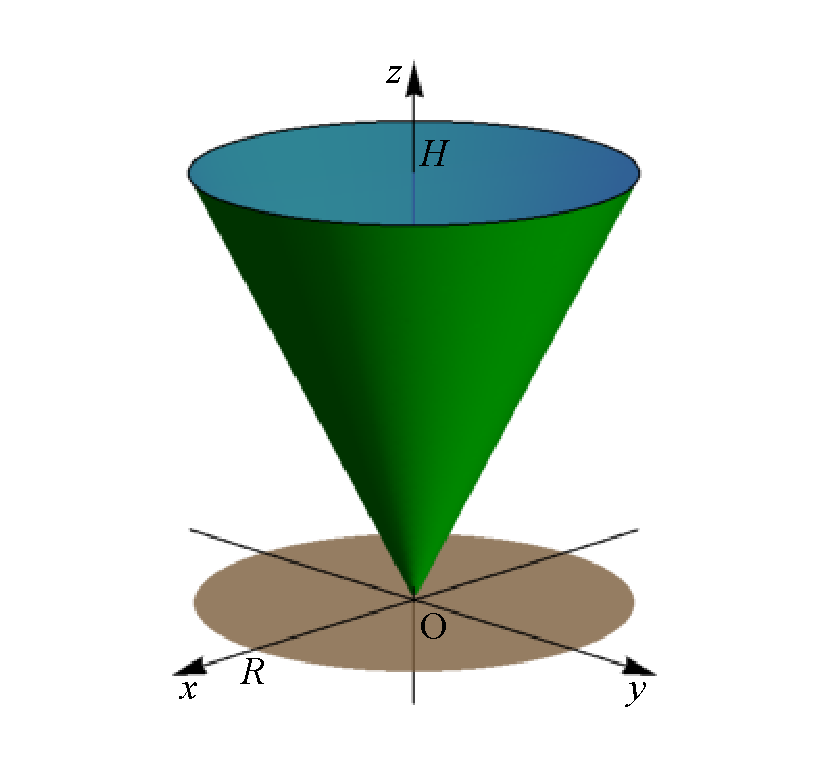
\includegraphics[height=0.7\textheight]{Figures21/Fig12-C-3.pdf}
\end{center}
\caption{第12章补充题 3.题图示}
\label{12-C-3}
\end{figure}

解:以该圆锥体的顶点为坐标原点,该圆锥体的旋转轴为$z$轴,建立空间直角坐标系,使该圆锥体在$xOy$平面上方,该圆锥体占据的空间区域可表示为$\Omega=\Set{(x,y,z)}{\frac HR\sqrt{x^2+y^2}\leqslant z\leqslant H,x^2+y^2\leqslant R^2}=\Set{(\theta,r,z)}{0\leqslant\theta\leqslant2\pi,0\leqslant r\leqslant R,\frac HRr\leqslant z\leqslant H}$根据对称性可知引力的$x$和$y$分量$F_x=F_y=0$,设该圆锥体的密度为$\rho$,则引力的$z$分量

$F_z=\varIIInt\Omega{\frac{G\rho m}{x^2+y^2+z^2}\frac z{\sqrt{x^2+y^2+z^2}}}xyz=\Int0{2\pi}{}\theta\Int0R{}r\Int{\frac HRr}H{\frac{G\rho m}{r^2+z^2}\frac z{\sqrt{r^2+z^2}}r}z\\
=2\pi G\rho m\Int0R{}r\Int{\frac HRr}H{\frac{rz}{(r^2+z^2)^{\frac32}}}z=2\pi G\rho m\Int0R{\frac12r\frac1{1-\frac32}(r^2+z^2)^{-\frac32+1}\big|_{\frac HRr}^H}r\\
=2\pi G\rho m\Int0R{r(\frac1{\sqrt{r^2+\frac{H^2}{R^2}r^2}}-\frac1{\sqrt{r^2+H^2}})}r=2\pi G\rho m\Int0R{(\frac1{\sqrt{1+\frac{H^2}{R^2}}}-\frac r{\sqrt{r^2+H^2}})}r\\
=2\pi G\rho m(\frac1{\sqrt{1+\frac{H^2}{R^2}}}r-\frac12\cdot\frac1{1-\frac12}\sqrt{r^2+H^2})\big|_0^R=2\pi G\rho m(\frac R{\sqrt{1+\frac{H^2}{R^2}}}-\sqrt{R^2+H^2}+H)\\
=2\pi G\rho m(H+\frac{R^2-R^2-H^2}{\sqrt{R^2+H^2}})=2\pi G\rho m(H-\frac{H^2}{\sqrt{R^2+H^2}})$,

故该圆锥体对位于其顶点处质量为$m$的质点的引力为$(0,0,2\pi G\rho m(H-\frac{H^2}{\sqrt{R^2+H^2}}))$.

(2)该圆锥体关于它的中心轴的转动惯量

$J_z=\varIIInt\Omega{(x^2+y^2)\rho}xyz=\Int0{2\pi}{}\theta\Int0R{}r\Int{\frac HRr}H{r^2\rho\cdot r}z=2\pi\rho\Int0R{r^3(H-\frac HRr)}r\\
=2\pi\rho(\frac14Hr^4-\frac15\frac HRr^5)\big|_0^R=2\pi\rho(\frac14HR^4-\frac15HR^4)=\frac1{10}\pi\rho HR^4$.

\item计算积分$\varIInt D{(x^2+y^2)^{\frac12}}xy$,其中$D=\Set{(x,y)}{0\leqslant x,y\leqslant a}$.

\begin{figure}[H]
\begin{center}
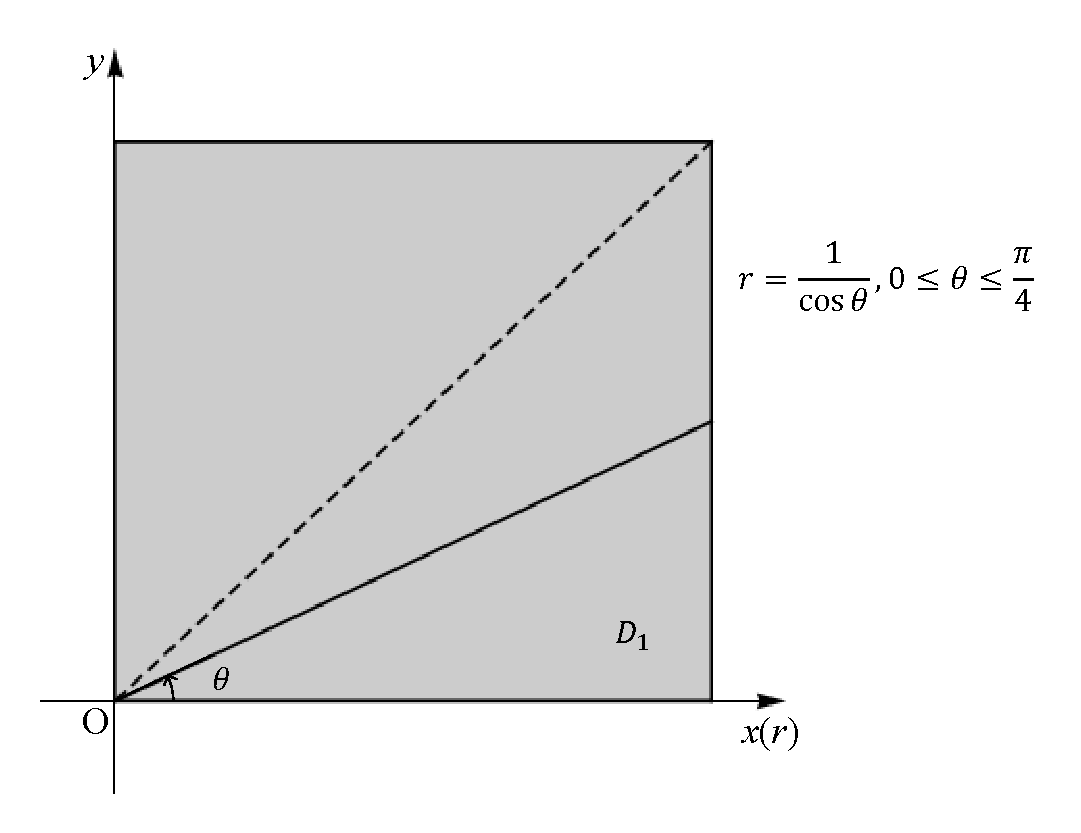
\includegraphics[height=0.3\textheight]{Figures21/Fig12-C-4.pdf}
\end{center}
\caption{第12章补充题 4.题图示}
\label{12-C-4}
\end{figure}

解:设$D_1=\Set{(x,y)}{0\leqslant x\leqslant1,0\leqslant y\leqslant x}=\Set{(r,\theta)}{0\leqslant\theta\leqslant\frac\pi4,0\leqslant r\leqslant\frac a{\cos\theta}}$,根据对称性可知

$\varIInt D{(x^2+y^2)^{\frac12}}xy=2\varIInt{D_1}{(x^2+y^2)^{\frac12}}xy=2\Int0{\frac\pi4}{}\theta\Int0{\frac a{\cos\theta}}{r\cdot r}r=2\Int0{\frac\pi4}{\frac13r^3\big|_0^{\frac a{\cos\theta}}}\theta\\
=2\Int0{2\pi}{\frac13\frac{a^3}{\cos^3\theta}}\theta=\frac23a^3\Int0{\frac\pi4}{\sec^3\theta}\theta=\frac23a^3\Int0{\frac\pi4}{\sec\theta}{\tan\theta}=\frac23a^3(\sec\theta\tan\theta\big|_0^{\frac\pi4}-\Int0{\frac\pi4}{\tan\theta}{\sec\theta})\\
=\frac23a^3(\sqrt2-\Int0{\frac\pi4}{\tan^2\theta\sec\theta}\theta)=\frac23a^3[\sqrt2-\Int0{\frac\pi4}{(\sec^2\theta-1)\sec\theta}\theta]\\
=\frac23a^3[\sqrt2-\Int0{\frac\pi4}{(\sec^3\theta-\sec\theta)}\theta]=\frac23a^3(\sqrt2-\Int0{\frac\pi4}{\sec^3\theta}\theta+\Int0{\frac\pi4}{\sec\theta}\theta)\\
=\frac{\frac23a^3}{\frac23a^3+\frac23a^3}(\frac23\sqrt2a^3+\frac23a^3\Int0{\frac\pi4}{\sec\theta}\theta)=\frac12(\frac23\sqrt2a^3+\frac23a^3\ln|\tan\theta+\sec\theta|\big|_0^{\frac\pi4})\\
=\frac13a^3[\sqrt2+\ln(1+\sqrt2)]$.

\item设$t>0,f(x)$在$[0,1]$上连续,求证$\Int0t{}x\Int0x{}y\Int0y{f(x)f(y)f(z)}z=\frac16(\Int0t{f(s)}s)^3$.

证明:方法1:设$F(x)=\Int0x{f(s)}s$,则
\[\begin{split}
&\Int0t{}x\Int0x{}y\Int0y{f(x)f(y)f(z)}z=\Int0t{f(x)}x\Int0x{f(y)}y\Int0y{f(z)}z\\
=&\Int0t{f(x)}x\Int0x{f(y)}y\Int0y{}{F(z)}=\Int0t{f(x)}x\Int0x{f(y)[F(y)-F(0)]}y\\
=&\Int0t{f(x)}x\Int0x{f(y)F(y)}y=\Int0t{f(x)}x\Int0x{F(y)}{F(y)}\\
=&\Int0t{f(x)\{\frac12[F(x)]^2-[F(0)]^2\}}x=\frac12\Int0t{[F(x)]^2}{F(x)}=\frac16[F(x)]^3\big|_0^t=\frac16[F(t)]^3\\
=&\frac16(\Int0t{f(s)}s)^3.
\end{split}\]
方法2:记$\varphi(y)=(\Int0y{f(z)}z)^2$,则$\varphi'(y)=2f(y)\Int0y{f(z)}z$. 于是

\[\begin{split}
\Int0x{}y\Int0y{f(y)f(z)}z&=\Int0x{}y[f(y)\Int0y{f(z)}z]=\frac12\Int0x{\varphi'y}y=\frac12\Int0x{}{\varphi(y)}=\frac12\varphi(x)\\
&=\frac12(\Int0x{f(s)}s)^2,
\end{split}\]

\[\begin{split}
\Int0t{}x\Int0x{}y\Int0y{f(x)f(y)f(z)}z&=\frac12\Int0t{}x[f(x)(\Int0x{f(s)}s)^2]=\frac16\Int0t{}{(\Int0x{f(s)}s)^3}\\
&=\frac16(\Int0t{f(s)}s)^3.
\end{split}\]

\item计算$\LInt L{(x^{\frac43}+y^{\frac43})}l$,其中$L$为星形线$x^{\frac23}+y^{\frac23}=a^{\frac23}(a>0)$.

\begin{figure}[H]
\begin{center}
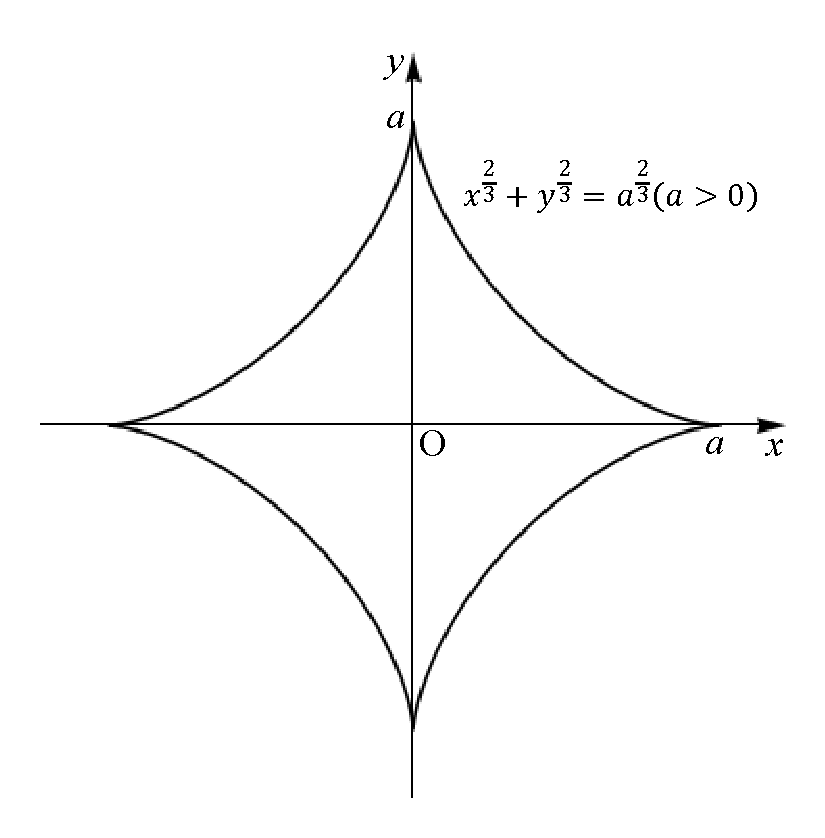
\includegraphics[height=0.3\textheight]{Figures21/Fig12-C-6.pdf}
\end{center}
\caption{第12章补充题 6.题图示}
\label{12-C-6}
\end{figure}

解:$L$的参数方程可表示为$\begin{cases}
x=a\cos^3\theta,\\
y=a\sin^3\theta,
\end{cases}0\leqslant\theta\leqslant2\pi$,

$\therefore\LInt L{(x^{\frac43}+y^{\frac43})}l=\Int0{2\pi}{(a^{\frac43}\cos^4\theta+a^{\frac43}\sin^4\theta)\sqrt{[(a\cos^3\theta)']^2+[(a\sin^3\theta)']^2}}\theta\\
=\Int0{2\pi}{(a^{\frac43}\cos^4\theta+a^{\frac43}\sin^4\theta)\sqrt{[-3a\cos^2\theta\sin\theta]^2+[3a\sin^2\theta\cos\theta]^2}}\theta\\
=\Int0{2\pi}{(a^{\frac43}\cos^4\theta+a^{\frac43}\sin^4\theta)\sqrt{9a^2\cos^2\theta\sin^2\theta}}\theta=4\Int0{\frac\pi2}{(a^{\frac43}\cos^4\theta+a^{\frac43}\sin^4\theta)\sqrt{9a^2\cos^2\theta\sin^2\theta}}\theta\\
=4\Int0{\frac\pi2}{(a^{\frac43}\cos^4\theta+a^{\frac43}\sin^4\theta)3a\cos\theta\sin\theta}\theta=12a^{\frac73}\Int0{\frac\pi2}{(\cos^5\theta\sin\theta+\sin^5\theta\cos\theta)}\theta\\
=12a^{\frac73}(\Int0{\frac\pi2}{\cos^5\theta\sin\theta}\theta+\Int0{\frac\pi2}{\sin^5\theta\cos\theta}\theta)=12a^{\frac73}(-\frac16\cos^6\theta\big|_0^{\frac\pi2}+\frac16\sin^6\theta\big|_0^{\frac\pi2})\\
=4a^{\frac73}$.

\item设$f(u)$是连续函数,$D=\Set{(x,y)}{x^2+y^2\leqslant a^2}$. 试求
\[
\varIInt D{\frac{af(x)+bf(y)}{f(x)+f(y)}}xy.
\]
解:$\because$积分域$D$关于$y=x$对称,且在关于$y=x$的对称点$(x,y)$和$(x',y')=(y,x)$处\\
$\frac{f(x')}{f(x')+f(y')}=\frac{f(y)}{f(y)+f(x)}$,

$\therefore\varIInt D{\frac{f(x)}{f(x)+f(y)}}xy=\varIInt D{\frac{f(y)}{f(x)+f(y)}}xy=\frac12\varIInt D{\frac{f(x)+f(y)}{f(x)+f(y)}}xy=\frac12\varIInt D{}xy=\frac12\pi a^2$,

$\therefore\varIInt D{\frac{af(x)+bf(y)}{f(x)+f(y)}}xy=a\varIInt D{\frac{f(x)}{f(x)+f(y)}}xy+b\varIInt D{\frac{f(y)}{f(x)+f(y)}}xy=\frac{a+b}2\pi a^2$.

\item设$D=\Set{(x,y)}{|x|+|y|\leqslant1}$,将$\varIInt D{f(x+y)}xy$化为定积分.

\begin{figure}[H]
\begin{center}
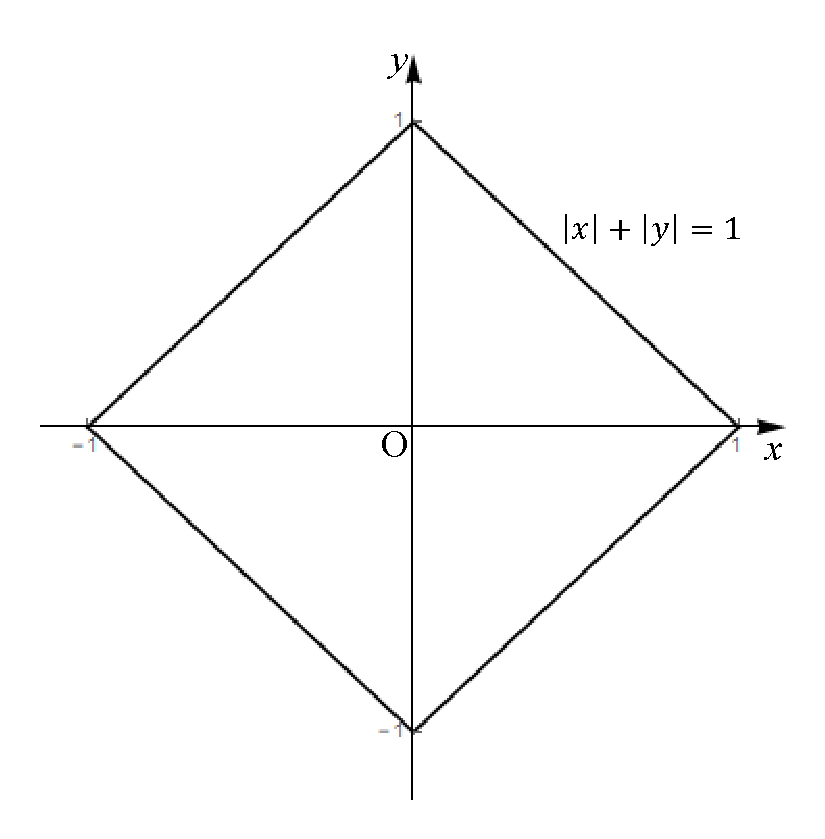
\includegraphics[height=0.3\textheight]{Figures21/Fig12-C-8.pdf}
\end{center}
\caption{第12章补充题 8.题图示}
\label{12-C-8}
\end{figure}

解:方法1:令$\begin{cases}
u=x+y,\\
v=x-y,
\end{cases}$则$D=\Set{(u,v)}{-1\leqslant u\leqslant 1,-1\leqslant v\leqslant 1}$,

$\frac{\mathrm D(u,v)}{\mathrm D(x,y)}=\begin{vmatrix}
1&1\\
1&-1
\end{vmatrix}=-2$,

$\therefore\varIInt D{f(x+y)}xy=\varIInt D{f(u)\frac1{|\frac{\mathrm D(u,v)}{\mathrm D(x,y)}|}}uv=\varIInt D{\frac12f(u)}uv=\frac12\Int{-1}1{}v\Int{-1}1{f(u)}u\\
=\Int{-1}1{f(u)}u$.

方法2:将重积分化为累次积分,有
\[
\varIInt{|x|+|y|\leqslant1}{f(x+y)}xy=\Int{-1}0{}x\Int{-1-x}{1+x}{f(x+y)}y+\Int01{}x\Int{-1+x}{1-x}{f(x+y)}y,
\]
令$x+y=u$,
\[\begin{split}
\text{上式}&=\Int{-1}0{}x\Int{-1}{1+2x}{f(u)}u+\Int01{x}\Int{2x-1}1{f(u)}u\\
&=\Int{-1}1{f(u)}u\Int{\frac{u-1}2}{\frac{u+1}2}{}x=\Int{-1}1{f(u)}u.
\end{split}\]

\item设一元函数$f$连续,$\Omega_t=\Set{(x,y,z)}{x^2+y^2\leqslant t^2,0\leqslant z\leqslant h}$. 令$F(t)=\IIInt{\Omega_t}{[z^2+f(x^2+y^2)]}V$,试求$\frac{\md F}{\md t}$和$\LIM t0\frac{F(t)}{t^2}$.

解:$F(t)=\varIIInt{\Omega_t}{[z^2+f(x^2+y^2)]}xyz=\Int0{2\pi}{}\theta\Int0t{}r\Int0h{[z^2+f(r^2)]r}z\\
=2\pi\Int0t{[\frac13rz^3+rf(r^2)z]\big|_0^h}r=2\pi\Int0t{[\frac13h^3r+hrf(r^2)]}r$,

$\therefore\frac{\mathrm dF}{\mathrm dt}=\frac{2\pi}3h^3t+2\pi htf(t^2)$,

$\therefore\LIM t0\frac1{t^2}F(t)=\LIM t0\frac{\frac{\mathrm dF}{\mathrm dt}}{2t}=\LIM t0\frac{2\pi[\frac13h^3t+htf(t^2)]}{2t}=\LIM t0\pi[\frac13h^3+hf(t^2)]=\frac\pi3h^3+\pi hf(0)$.

\item计算下列积分:\\
(1)$\IIInt\Omega{(ax+by+cz)^2}V$,其中$\Omega=\Set{(x,y,z)}{x^2+y^2+z^2\leqslant R^2}$;\\
(2)$\IIInt\Omega{(\frac{x^2}{a^2}+\frac{y^2}{b^2}+\frac{z^2}{c^2})}V$,其中$\Omega=\Set{(x,y,z)}{\frac{x^2}{a^2}+\frac{y^2}{b^2}+\frac{z^2}{c^2}\leqslant1}$.

解:(1)方法1:由对称性可知

$\IIInt\Omega{(ax+by+cz)^2}V=\IIInt\Omega{(a^2x^2+b^2y^2+c^2z^2+2abxy+2acxz+2bcyz)}V\\
=\IIInt\Omega{(a^2x^2+b^2y^2+c^2z^2)}V=(a^2+b^2+c^2)\IIInt\Omega{z^2}V\\
=(a^2+b^2+c^2)\varIIInt\Omega{r^2\cos^2\varphi\cdot r^2\sin\varphi}\theta\varphi r\\
=(a^2+b^2+c^2)\Int0{2\pi}{}\theta\Int0R{r^4}r\Int0\pi{\cos^2\varphi\sin\varphi}\varphi\\
=\frac25\pi R^5(a^2+b^2+c^2)(-\frac13\cos^3\varphi)\big|_0^\pi=\frac4{15}\pi R^5(a^2+b^2+c^2)$.

方法2:$\IIInt\Omega{(ax+by+cz)^2}V=\IIInt\Omega{(a^2x^2+b^2y^2+c^2z^2+2abxy+2acxz+2bcyz)}V\\
=\IIInt\Omega{(a^2x^2+b^2y^2+c^2z^2)}V=(a^2+b^2+c^2)\IIInt\Omega{z^2}V=\frac13(a^2+b^2+c^2)\IIInt\Omega{(x^2+y^2+z^2)}V\\
=\frac13(a^2+b^2+c^2)\Int0{2\pi}{}\theta\Int0\pi{}\varphi\Int0R{r^2\cdot r^2\sin\varphi}r=\frac23\pi(a^2+b^2+c^2)\Int0\pi{\sin\varphi}\varphi\Int0R{r^4}r\\
=\frac23\pi(a^2+b^2+c^2)(-\cos\varphi)\big|_0^\pi\frac15r^5\big|_0^R=\frac4{15}\pi R^5(a^2+b^2+c^2)$.

(2)令$\begin{cases}
x=au,\\
y=bv,\\
z=cw,
\end{cases}$则$\Omega=\Set{(u,v,w)}{u^2+v^2+w^2\leqslant1}$,

$\frac{\mathrm D(x,y,z)}{\mathrm D(u,v,w)}=\begin{vmatrix}
a&0&0\\
0&b&0\\
0&0&c
\end{vmatrix}=abc$,

$\therefore\IIInt\Omega{(\frac{x^2}{a^2}+\frac{y^2}{b^2}+\frac{z^2}{c^2})}V=\varIIInt\Omega{(u^2+v^2+w^2)|\frac{\mathrm D(u,v,w)}{\mathrm D(x,y,z)}|}uvw=abc\varIIInt\Omega{(u^2+v^2+w^2)}uvw\\
=abc\frac4{15}\pi 1^4(1^2+1^2+1^2)=\frac45\pi abc$.

\end{enumerate}
\subsection{习题13.1解答}
\begin{enumerate}
\item验证梯度算子$\bm\nabla$的下列性质,其中$\alpha,\beta$为任意常数,$f,g$为任意可微函数:\\
(1)$\bm\nabla(\alpha f+\beta g)=\alpha\bm\nabla+\beta\bm\nabla g$;\\
(2)$\bm\nabla(fg)=g\bm\nabla f+f\bm\nabla g$;\\
(3)$\bm\nabla(\frac fg)=\frac{g\bm\nabla f-f\bm\nabla g}{g^2}$(在$g$不等于零处成立).

证明:(1)\[\begin{split}
\bm\nabla(\alpha f+\beta g)&=(\pp{}x\bm i+\pp{}y\bm j+\pp{}z\bm k)(\alpha f+\beta g)\\
&=\pp{(\alpha f+\beta g)}x\bm i+\pp{(\alpha f+\beta g)}y\bm j+\pp{(\alpha f+\beta g)}z\bm k\\
&=(\alpha\pp fx+\beta\pp gx)\bm i+(\alpha\pp fy+\beta\pp gy)\bm j+(\alpha\pp fz+\beta\pp gz)\bm k\\
&=\alpha(\pp fx\bm i+\pp fy\bm j+\pp fz\bm k)+\beta(\pp gx\bm i+\pp gy\bm j+\pp gz\bm k)\\
&=\alpha\bm\nabla f+\beta\bm\nabla g.
\end{split}\]
(2)\[\begin{split}
\bm\nabla(fg)&=(\pp{}x\bm i+\pp{}y\bm j+\pp{}z\bm k)(fg)\\
&=\pp{(fg)}x\bm i+\pp{(fg)}y\bm j+\pp{(fg)}z\bm k\\
&=(g\pp fx+f\pp gx)\bm i+(g\pp fy+f\pp gy)\bm j+(g\pp fz+f\pp gz)\bm k\\
&=g(\pp fx\bm i+\pp fy\bm j+\pp fz\bm k)+f(\pp gx\bm i+\pp gy\bm j+\pp gz\bm k)\\
&=g\bm\nabla f+f\bm\nabla g.
\end{split}\]
(3)\[\begin{split}
\bm\nabla(\frac fg)&=(\pp{}x\bm i+\pp{}y\bm j+\pp{}z\bm k)(\frac fg)\\
&=\pp{}x(\frac fg)\bm i+\pp{}y(\frac fg)\bm j+\pp{}z(\frac fg)\bm k\\
&=\frac{g\pp fx-f\pp gx}{g^2}\bm i+\frac{g\pp fy-f\pp gy}{g^2}\bm j+\frac{g\pp fz-f\pp gz}{g^2}\bm k\\
&=\frac{g(\pp fx\bm i+\pp fy\bm j+\pp fz\bm k)-f(\pp gx\bm i+\pp gy\bm j+\pp gz\bm k)}{g^2}\\
&=\frac{g\bm\nabla f-f\bm\nabla g}{g^2}.
\end{split}\]
\item验证散度算子的下列性质(其中$f$为函数,$\bm u,\bm v$是向量场):
\[\bm\nabla\bm\cdot(\bm u\times\bm v)=-\bm u\bm\cdot\bm\nabla\times\bm v+\bm v\bm\cdot\bm\nabla\times\bm u.\]
证明:\[\begin{split}
\bm\nabla\bm\cdot(\bm u\times\bm v)&=(\pp{}x\bm i+\pp{}y\bm j+\pp{}z\bm k)\bm\cdot\begin{vmatrix}
\bm i&\bm j&\bm k\\
u_1(x,y,z)&u_2(x,y,z)&u_3(x,y,z)\\
v_1(x,y,z)&v_2(x,y,z)&v_3(x,y,z)
\end{vmatrix}\\
&=(\pp{}x\bm i+\pp{}y\bm j+\pp{}z\bm k)\bm\cdot[(u_2v_3-u_3v_2)\bm i+(u_3v_1-u_1v_3)\bm j+(u_1v_2-u_2v_2)\bm k]\\
&=\pp{(u_2v_3-u_3v_2)}x+\pp{(u_3v_1-u_1v_3)}y+\pp{(u_1v_2-u_2v_1)}z\\
&=\pp{u_2}xv_3+u_2\pp{v_3}x-\pp{u_3}xv_2-u_3\pp{v_2}x\\
&+\pp{u_3}yv_1+u_3\pp{v_1}y-\pp{u_1}yv_3-u_1\pp{v_3}y\\
&+\pp{u_1}zv_2+u_1\pp{v_2}z-\pp{u_2}zv_1-u_2\pp{v_1}z\\
&=u_1(\pp{v_2}z-\pp{v_3}y)+u_2(\pp{v_3}x-\pp{v_1}z)+u_3(\pp{v_1}y-\pp{v_2}x)\\
&+v_1(\pp{u_3}y-\pp{u_2}z)+v_2(\pp{u_1}z-\pp{u_3}x)+v_3(\pp{u_2}x-\pp{u_1}y)\\
&=-u_1(\pp{v_3}y-\pp{v_2}z)-u_2(\pp{v_1}z-\pp{v_3}x)-u_3(\pp{v_2}x-\pp{v_1}y)\\
&\quad+v_1(\pp{u_3}y-\pp{u_2}z)+v_2(\pp{u_1}z-\pp{u_3}x)+v_3(\pp{u_2}x-\pp{u_1}y)\\
&=-(u_1\bm i+u_2\bm j+u_3\bm k)\bm\cdot[(\pp{v_3}y-\pp{v_2}z)\bm i+(\pp{v_1}z-\pp{v_3}x)\bm j+(\pp{v_3}x-\pp{v_1}y)\bm k]\\
&\quad+(v_1\bm i+v_2\bm j+v_3\bm k)\bm\cdot[(\pp{u_3}y-\pp{u_2}z)\bm i+(\pp{u_1}z-\pp{u_3}x)\bm j+(\pp{u_2}x-\pp{u_1}y)\bm k]\\
&=-(u_1\bm i+u_2\bm j+u_3\bm k)\bm\cdot\begin{vmatrix}
\bm i&\bm j&\bm k\\
\pp{}x&\pp{}y&\pp{}z\\
v_1&v_2&v_3
\end{vmatrix}+(v_1\bm i+v_2\bm j+v_3\bm k)\bm\cdot\begin{vmatrix}
\bm i&\bm j&\bm k\\
\pp{}x&\pp{}y&\pp{}z\\
u_1&u_2&u_3
\end{vmatrix}\\
&=-\bm u\bm\cdot(\bm\nabla\times\bm v)+\bm v\bm\cdot(\bm\nabla\times\bm u)
\end{split}\]
%\[\begin{split}
%&-\bm u\bm\cdot(\bm\nabla\times\bm v)+\bm v\bm\cdot(\bm\nabla\times\bm u)\\
%=&-(u_1\bm i+u_2\bm j+u_3\bm k)\bm\cdot\begin{vmatrix}
%\bm i&\bm j&\bm k\\
%\pp{}x&\pp{}y&\pp{}z\\
%v_1&v_2&v_3
%\end{vmatrix}+(v_1\bm i+v_2\bm j+v_3\bm k)\bm\cdot\begin{vmatrix}
%\bm i&\bm j&\bm k\\
%\pp{}x&\pp{}y&\pp{}z\\
%u_1&u_2&u_3
%\end{vmatrix}\\
%=&-(u_1\bm i+u_2\bm j+u_3\bm k)\bm\cdot[(\pp{v_3}y-\pp{v_2}z)\bm i+(\pp{v_1}z-\pp{v_3}x)\bm j+(\pp{v_3}x-\pp{v_1}y)\bm k]\\
%&+(v_1\bm i+v_2\bm j+v_3\bm k)\bm\cdot[(\pp{u_3}y-\pp{u_2}z)\bm i+(\pp{u_1}z-\pp{u_3}x)\bm j+(\pp{u_2}x-\pp{u_1}y)\bm k]\\
%=&-u_1(\pp{v_3}y-\pp{v_2}z)-u_2(\pp{v_1}z-\pp{v_3}x)-u_3(\pp{v_3}x-\pp{v_1}y)\\
%&+v_1(\pp{u_3}y-\pp{u_2}z)+v_2(\pp{u_1}z-\pp{u_3}x)+v_3(\pp{u_2}x-\pp{u_1}y)
%\end{split}\]
\item设$\bm r=x\bm i+y\bm j+z\bm k,r=\sqrt{x^2+y^2+z^2}$:\\
(1)设$f(u)$为可微函数,求$\bm\nabla f(r)$;\\
(2)设$\bm F=f(r)\bm r$,求证$\bm\nabla\times\bm F\equiv\bm0$. 又问当$f$满足什么条件时,$\bm\nabla\bm\cdot\bm F=0$?

解:(1)\[\begin{split}
\bm\nabla f(r)&=\pp{f(r)}x\bm i+\pp{f(r)}y\bm j+\pp{f(r)}z\bm k\\
&=f'(r)\pp rx\bm i+f'(r)\pp ry\bm j+f'(r)\pp rz\bm k=f'(r)(\pp rx\bm i+\pp ry\bm j+\pp rz\bm k)\\
&=f'(r)(\frac x{\sqrt{x^2+y^2+z^2}}\bm i+\frac y{\sqrt{x^2+y^2+z^2}}\bm j+\frac z{\sqrt{x^2+y^2+z^2}}\bm k)\\
&=\frac{f'(r)}{\sqrt{x^2+y^2+z^2}}(x\bm i+y\bm j+z\bm k)=\frac{f'(r)}r\bm r.
\end{split}\]

(2)

i)证明:
\[\begin{split}
\bm\nabla\times\bm F&=\bm\nabla\times[f(r)\bm r]=\bm\nabla f(r)\times\bm r+f(r)\bm\nabla\times\bm r\\
&=\frac{f'(r)}r\bm r\times\bm r+f(r)\bm\nabla\times\bm r\\
&=0+f(r)\begin{vmatrix}
\bm i&\bm j&\bm k\\
\pp{}x&\pp{}y&\pp{}z\\
x&y&z
\end{vmatrix}\\
&=f(r)[(\pp zy-\pp yz)\bm i+(\pp xz-\pp zx)\bm j+(\pp yx-\pp xy)\bm k]\\
&=f(r)(0\bm i+0\bm j+0\bm k)=0.
\end{split}\]
ii)

$\because$
\[\begin{split}
\bm\nabla\bm\cdot\bm F&=\bm\nabla\bm\cdot[f(r)\bm r]=\bm\nabla f(r)\bm\cdot\bm r+f(r)\bm\nabla\bm\cdot\bm r=\frac{f'(r)}r\bm r\bm\cdot\bm r+f(r)(\pp xx+\pp yy+\pp zz)\\
&=\frac{\md f(r)}{\md r}r+3f(r)=0,
\end{split}\]
$\therefore$当$f(r)\neq0$时,$r\neq0$,
\[\frac{\md f(r)}{f(r)}=-3\frac{\md r}r,\]
$\therefore$
\[
\ln|f(r)|=-3\ln|r|+C_1,
\]
$\therefore$
\[
f(r)=\frac C{r^3},\text{$C$为任意常数}.
\]
\item验证旋度算子的下列基本公式:\\
(1)$\bm\nabla\times(\alpha\bm u+\beta\bm v)=\alpha\bm\nabla\times\bm u+\beta\bm\nabla\times\bm v$;\\
(2)$\bm\nabla\times(\bm\nabla f)=\bm0$;\\
(3)$\bm\nabla\bm\cdot(\bm\nabla\times\bm v)=0$.

证明:(1)\[\begin{split}
\bm\nabla\times(\alpha\bm u+\beta\bm v)&=\bm\nabla\times(\alpha u_1\bm i+\alpha u_2\bm j+\alpha u_3\bm k+\beta v_1\bm i+\beta v_2\bm j+\beta v_3\bm k)\\
&=\bm\nabla\times[(\alpha u_1+\beta v_1)\bm i+(\alpha u_2+\beta v_2)\bm j+(\alpha u_3+\beta v_3)\bm k]\\
&=\pp{(\alpha u_1+\beta v_1)}x+\pp{(\alpha u_2+\beta v_2)}y+\pp{(\alpha u_3+\beta v_3)}z\\
&=\alpha\pp{u_1}x+\beta\pp{v_1}x+\alpha\pp{u_2}y+\beta\pp{v_2}y+\alpha\pp{u_3}z+\beta\pp{v_3}z\\
&=\alpha(\pp{u_1}x+\pp{u_2}y+\pp{u_3}z)+\beta(\pp{v_1}x+\pp{v_2}y+\pp{v_3}z)\\
&=\alpha\bm\nabla\cdot\bm u+\beta\bm\nabla\cdot\bm v.
\end{split}\]
(2)当$f\in C^2$时
\[\begin{split}
\bm\nabla\times(\bm\nabla f)&=\bm\nabla\times(\pp fx\bm i+\pp fy\bm j+\pp fz\bm k)=\begin{vmatrix}
\bm i&\bm j&\bm k\\
\pp{}x&\pp{}y&\pp{}z\\
\pp fx&\pp fy&\pp fz
\end{vmatrix}\\
&=(\frac{\partial^2f}{\partial x\partial z}-\frac{\partial^2f}{\partial z\partial x})\bm i+(\frac{\partial^2f}{\partial z\partial x}-\frac{\partial^2f}{\partial x\partial z})\bm j+(\frac{\partial^2f}{\partial x\partial y}-\frac{\partial^2f}{\partial y\partial x})\bm k\\
&=0\bm i+0\bm j+0\bm k=\bm0.
\end{split}\]
(3)当$\bm v\in C^2$时
\[\begin{split}
\bm\nabla\bm\cdot(\bm\nabla\times\bm v)&=(\pp{}x\bm i+\pp{}y\bm j+\pp{}z\bm k)\bm\cdot\begin{vmatrix}
\bm i&\bm j&\bm k\\
\pp{}x&\pp{}y&\pp{}z\\
v_1(x,y,z)&v_2(x,y,z)&v_3(x,y,z)
\end{vmatrix}\\
&=(\pp{}x\bm i+\pp{}y\bm j+\pp{}z\bm k)\bm\cdot[(\pp{v_3}y-\pp{v_2}z)\bm i+(\pp{v_1}z-\pp{v_3}x)\bm j+(\pp{v_2}x-\pp{v_1}y)\bm k]\\
&=(\frac{\partial^2 v_3}{\partial x\partial y}-\frac{\partial^2 v_2}{\partial x\partial z})+(\frac{\partial^2 v_1}{\partial y\partial  z}-\frac{\partial^2 v_3}{\partial y\partial x})+(\frac{\partial^2 v_2}{\partial z\partial x}-\frac{\partial^2 v_1}{\partial z\partial y})\\
&=(\frac{\partial^2 v_3}{\partial x\partial y}-\frac{\partial^2 v_3}{\partial y\partial x})+(\frac{\partial^2 v_1}{\partial y\partial  z}-\frac{\partial^2 v_1}{\partial z\partial y})+(\frac{\partial^2 v_2}{\partial z\partial x}-\frac{\partial^2 v_2}{\partial x\partial z})\\
&=0.
\end{split}\]
\item求下列向量场的散度:\\
(1)$\bm v=xyz(x\bm i+y\bm j+z\bm k)$;\\
(2)$\bm v=(x\bm i+y\bm j+z\bm k)\times\bm c$;\\
(3)$\bm v=[(x\bm i+y\bm j+z\bm k)\bm\cdot\bm c](x\bm i+y\bm j+z\bm k)$(其中$\bm c$为常值向量).

解:(1)\[\begin{split}
\bm\nabla\bm\cdot\bm v&=\bm\nabla(xyz)\bm\cdot(x\bm i+y\bm j+z\bm k)+xyz\bm\nabla\bm\cdot(x\bm i+y\bm j+z\bm k)\\
&=(yz\bm i+xz\bm j+xy\bm k)\bm\cdot(x\bm i+y\bm j+z\bm k)+xyz(\pp xx+\pp yy+\pp zz)\\
&=xyz+xyz+xyz+3xyz=6xyz.
\end{split}\]
(2)\[\begin{split}
\bm\nabla\bm\cdot\bm v&=\bm c\bm\cdot[\bm\nabla\times(x\bm i+y\bm j+z\bm k)]-(x\bm i+y\bm j+z\bm k)\cdot(\bm\nabla\times\bm c)\\
&=\bm c\bm\cdot\begin{vmatrix}
\bm i&\bm j&\bm k\\
\pp{}x&\pp{}y&\pp{}z\\
x&y&z
\end{vmatrix}-(x\bm i+y\bm j+z\bm k)\bm\cdot\bm0\\
&=\bm c\bm\cdot[(\pp zy-\pp yz)\bm i+(\pp xz-\pp zx)\bm j+(\pp yx-\pp xy)\bm k]-0\\
&=\bm c\bm\cdot\bm0-0=0.
\end{split}\]
(3)记$\bm c=(c_1,c_2,c_3)$
\[\begin{split}
\bm\nabla\bm\cdot\bm v&=[(x\bm i+y\bm j+z\bm k)\bm\cdot\bm c]\bm\nabla\bm\cdot(x\bm i+y\bm j+z\bm k)+(x\bm i+y\bm j+z\bm k)\bm\cdot\bm\nabla[(x\bm i+y\bm j+z\bm k)\bm\cdot\bm c]\\
&=[(x\bm i+y\bm j+z\bm k)\bm\cdot\bm c](\pp xx+\pp yy+\pp zz)+(x\bm i+y\bm j+z\bm k)\bm\cdot\bm\nabla(c_1x+c_2y+c_3z)\\
&=3[(x\bm i+y\bm j+z\bm k)\bm\cdot\bm c]+(x\bm i+y\bm j+z\bm k)\bm\cdot(c_1\bm i+c_2\bm j+c_3\bm k)\\
&=3[(x\bm i+y\bm j+z\bm k)\bm\cdot\bm c]+(x\bm i+y\bm j+z\bm k)\bm\cdot\bm c\\
&=4[(x\bm i+y\bm j+z\bm k)\bm\cdot\bm c.
\end{split}\]
\item求下列向量场的旋度:\\
(1)$\bm v=y^2z\bm i+z^2x\bm j+x^2y\bm k$;\\
(2)$\bm v=f(\sqrt{x^2+y^2+z^2})\bm c$(其中$\bm c$)为常值向量.

解:(1)\[\begin{split}
\bm\nabla\times\bm v=\begin{vmatrix}
\bm i&\bm j&\bm k\\
\pp{}x&\pp{}y&\pp{}z\\
y^2z&z^2x&x^2y
\end{vmatrix}=(x^2-2xz)\bm i+(y^2-2xy)\bm j+(z^2-2yz)\bm k.
\end{split}\]
(2)\[\begin{split}
\bm\nabla\times\bm v&=\bm\nabla\times[f(\sqrt{x^2+y^2+z^2})\bm c]\\
&=\bm\nabla f(\sqrt{x^2+y^2+z^2})\times\bm c+f(\sqrt{x^2+y^2+z^2})\bm\nabla\times\bm c\\
&=f'(\sqrt{x^2+y^2+z^2})(\frac x{\sqrt{x^2+y^2+z^2}}\bm i+\frac y{\sqrt{x^2+y^2+z^2}}\bm j+\frac z{\sqrt{x^2+y^2+z^2}}\bm k)\times\bm c+\bm0\\
&=\frac{f'(\sqrt{x^2+y^2+z^2})}{\sqrt{x^2+y^2+z^2}}(x\bm i+y\bm j+z\bm k)\times\bm c.
\end{split}\]
\end{enumerate}
\end{document}